\documentclass{beamer}

\usetheme{Boadilla}

\usepackage{hyperref}
\hypersetup{colorlinks=true}

\begin{document}

\title{Introduction to ROS} 
\author{Kurbakov Dmytro, Slonina Michal}

\date{11.10.2019}

\begin{frame}
\titlepage
\end{frame}

\begin{frame}
All slides are available here:

\url{https://github.com/project-omicron/robocar/}
\end{frame}

\begin{frame}{Table of contents}
\tableofcontents
\end{frame}

\section{History of ROS} 
\begin{frame}{Early years of ROS, ... - 2007}
\begin{tabular}{ll}
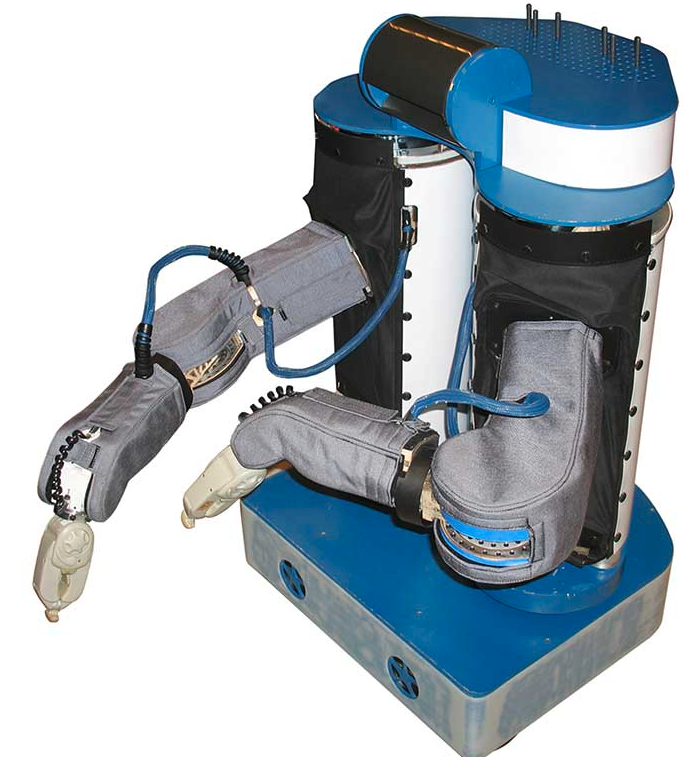
\includegraphics[scale=0.08]{images/pr1_clean} 
&
\begin{tabular}{l}
No single solution how to program robots \\
\\
Eric Berger and Keenan Wyrobek, PhD students at \\
Stanford, build PR1 (Personal Robot One) and began\\
to work on software from it, borrowing the best \\
practices from other early open source robotic \\
software frameworks \\
\\
Early funding of US\$50,000 was provided by Joanna \\
Hoffman and Alain Rossmann,  which supported the \\
development of the PR1
\end{tabular}
\end{tabular}
\end{frame}

\begin{frame}{Early years of ROS, 2007 - 2013}
\begin{tabular}{ll}
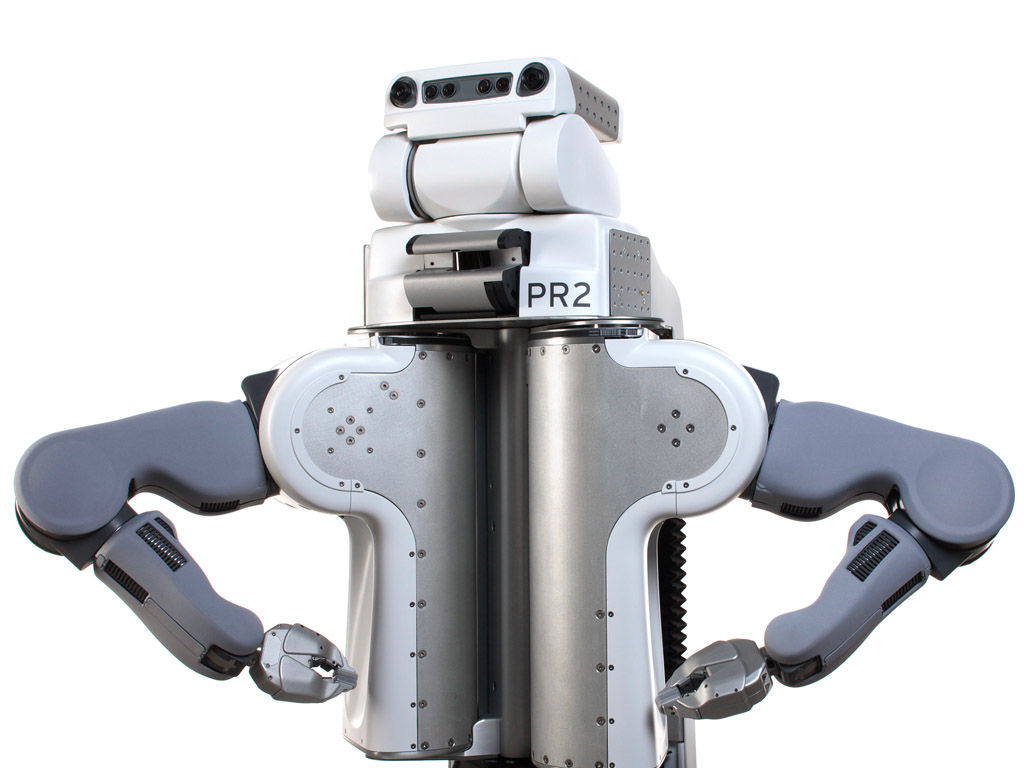
\includegraphics[scale=0.08]{images/pr2} 
&
\begin{tabular}{l}
PR2 was introduced\\
\\
Introduction of many packages\\
\\
First RVIZ documentation, first paper on ROS\\
\\
Initiation of the ROS.org website\\
\\
Release of ROS 1.0, in January 2010\\
\\
Creating the Open Source Robotics Foundation\\
\end{tabular}
\end{tabular}
\end{frame}

\begin{frame}{Early years of ROS, 2013 - now}
\begin{tabular}{ll}
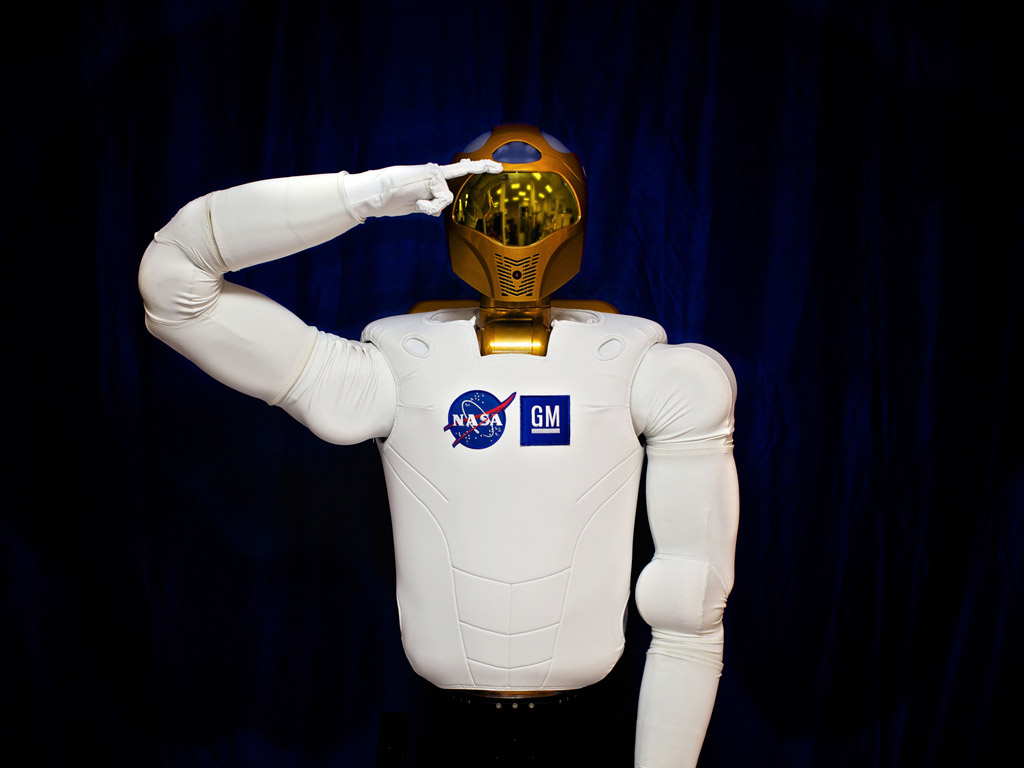
\includegraphics[scale=0.08]{images/robonaut} 
&
\begin{tabular}{l}
A new version of ROS every year\\
\\
ROSCons have occurred every year since 2012\\
\\
Robotnaut 2: forst ROS based robot in space\\
\\
ROS2 was released\\
\end{tabular}
\end{tabular}
\end{frame}

\section{Structure of ROS}
\subsection{Catkin workspace}
\begin{frame}{What is a workspace in ROS}
\textbf{Workspace} is the folder inside which you are going to be actively developing. Keeping things in a folder with connected development helps keep separation of development models
\vfill
\textbf{Catkin} is a low-level build system macros and infrastructure for ROS
\vfill
\textbf{Catkin workspace} is a folder where you modify, build, and install catkin packages
\vfill
For more information, check: \href{http://wiki.ros.org/catkin}{ROS catkin documantation}
\end{frame}

\begin{frame}{Introduction to catkin\_init\_workspace and catkin\_make}
\textbf{catkin\_init\_workspace} initializes a catkin workspace by creating a top level CMakeLists.txt
\vfill
\textbf{catkin\_make} is a convenience tool for building code in a catkin workspace. catkin\_make follows the standard layout of a catkin workspace
\end{frame}

\subsection{Node}
\begin{frame}{Robot architecture in ROS, example}
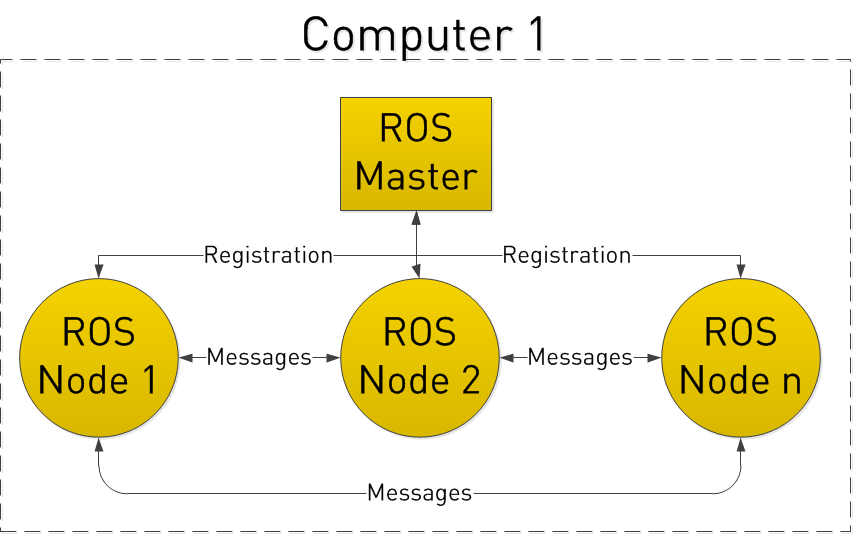
\includegraphics[scale=0.35]{images/ros}
\end{frame}

\begin{frame}{ROS Master}
The ROS Master provides naming and registration services to the rest of the nodes in the ROS system.

\begin{itemize}
\item Tracks publishers and subscribers nodes
\item Tracks topics
\item Tracks services
\item Provide parameter server\\
Shared, multi-variate dictionary, accessible via network APIs.\\
Nodes use this server to store and retrieve parameters at runtime.\\
\end{itemize}
\end{frame}

\begin{frame}{Publisher vs. Subscriber}
\textbf{Publisher}: Node that puts information to the topic
\vfill
\textbf{Subscriber}: Node that checkes if the information arrives to the topic. Once the information arrived, it can react correspondingly
\vfill
In ROS, every note can be a publisher, subscriber or both
\vfill
For more info, check \href{http://wiki.ros.org/ROS/Tutorials/WritingPublisherSubscriber\%28python\%29}{here}
\end{frame}

\subsection{Topic}
\begin{frame}{What is the topic in ROS}
\textbf{Topic} is a named buse over which nodes exchange messages
\vfill
Each topic is strongly typed by the ROS message type
\vfill
ROS currently supports TCP/IP-based and UDP-based message transport
\begin{enumerate}
\item TCPROS is the default transport used in ROS 
\item UDP-based transportis currently only supported in roscpp
\end{enumerate}
\end{frame}

\begin{frame}{Introduction to the command rostopic}
\textbf{rostopic} is a command-line tool for interacting with ROS topics
\vfill
Once you run the robot, you can see all available topics\\
\textit{rostopic list}
\vfill
Current value in the topic\\
\textit{rostopic echo /topic\_name}
\vfill
Information about the frequenze of the topic\\
\textit{rostopic hz /topic\_name}
\vfill
More information: \href{http://wiki.ros.org/rostopic}{ROS Topic}
\end{frame}

\subsection{Service}
\begin{frame}{What is the service in ROS}
Request/reply is done via a Service, which is defined by a pair of messages: one for the request and one for the reply.
\vfill
Services are defined using srv files.
\vfill
Generally saying: service is the RPC in ROS.
\end{frame}

\begin{frame}{Introduction to the command rosservice}
\textbf{rosservice} contains the rosservice command-line tool for listing and querying ROS Services
\vfill
List all the services that are currently available\\
\textit{rosservice list}
\vfill
Print information about specified service
\textit{rosservice info /rosout}
\vfill
Call a service from the command line\\
\textit{rosservice call /service\_name service-args}
\vfill
For more information: \href{http://wiki.ros.org/rosservice}{ROS Service}
\end{frame}

\begin{frame}{MUX}
\textit{mux} is a ROS node that subscribes to a set of incoming topics and republishes incoming data from one of them to another topic
\vfill
Example:\\
We use mix to switch from AI controller to human controller.
\vfill
More information and examples: \href{http://wiki.ros.org/topic_tools/mux}{ROS mux}
\end{frame}

\subsection{How to run the robot}
\begin{frame}{roscore and rosrun}
just explain the command
\end{frame}

\begin{frame}{roslaunch}
just explain the command
\end{frame}

\section{Introduction to Omicron}
\subsection{Team}
\begin{frame}{Active contributers}
Michal and Dmytro are cool guys who do the job!
\end{frame}

\subsection{Why Omicron}
\begin{frame}{Why should you use Omicron}
Omicron is awesome!
\end{frame}

\subsection{Packages}
\begin{frame}{High level description of nodes}
show a graph how the structure looks like
\end{frame}

\subsection{Topics}
\begin{frame}{Topics}
go through topics and who is doing what
\end{frame}

\subsection{Message types}
\begin{frame}{Ackermann message}
show the structire of the message
\end{frame}

\begin{frame}{Image}
show the structure of the message
\end{frame}

\section{Useful links}

\begin{frame}{What to know more?}
\href{https://spectrum.ieee.org/automaton/robotics/robotics-software/the-origin-story-of-ros-the-linux-of-robotics}{The Origin Story of ROS, the Linux of Robotics}\\
\href{https://www.ros.org/history/}{ROS History, ROS.org}\\
\href{https://en.wikipedia.org/wiki/Robot_Operating_System}{ROS, wiki page}\\
\href{http://wiki.ros.org/Industrial/Tutorials}{ROS Industrial}
\end{frame}

\begin{frame}{Q \& A}
Contacts
links to the repo
\end{frame}

\end{document}

